\begin{Example}[lifeboat1]{Lifeboats on the \emph{Titanic}}
We examine the question of who survived and why in the sinking of the \emph{RMS Titanic} in \secref{sec:mosaic-threeway} (\exref{ex:titanic}),
where we analyze a four-way table of the 2201 people on board (1316 passengers and 885 crew),
classified by Class, Sex, Age, and Survival.
A different \Dset\ which sheds some light on the same issues is
appropriate here.

After the disaster, the British Board of Trade launched several
inquiries, the most comprehensive of which resulted in the
\emph{Report on the Loss of the ``Titanic'' (S.S.)}
by Lord Mersey
\citep{Mersey:1912}.
Section 4 of this document contains a detailed account of the saving
and rescue of the passengers and crew who survived.
The \emph{Titanic} was outfitted with 20 boats, half on each of the
port and starboard sides,
 of which 14 were large
lifeboats with a capacity of 65, two were emergency boats designed for
40 persons, and the remaining four were collapsible boats capable of holding
47, a total capacity of 1178 (considered adequate at that time).
Two of the collapsible boats, lashed to the roof of the officers
quarters, were ineffectively launched and utilized as rafts after the ship sunk.
The report lists the time of launch and composition of the remaining 18 boats according to male passengers, women and children, and ``men of crew'',
as reported by witnesses.
The \Dset\ \texttt{lifeboat} (see \datref{dat:lifeboat})
contains the data listed on p. 38 of that report.%
\footnote{The ``data'' lists a total of 854 in 18 boats, although only
712 were in fact saved.  Mersey notes ``it is obvious that these figures
are quite unreliable''.  Allowing for 60 people rescued from the water,
only 652 could have left in the boats \citep[p. 39]{Mersey:1912}.
We present an alternative \Dset, \pname{LIFEBOA2}, in \datref{dat:lifeboat},
based on more conservative and historically accurate informatio.}

Of interest here is the composition of the boats by these three categories
and according to the launching of the boats from the port or starboard
side, which can be shown in a trilinear display
using the following statements.
The parameter \pname{idsubset = men>.1} is used to label only boats
in which the proportion of male passengers exceeded 10\%.
(The values of variables have been scaled to sum to 1.0 for each observation
at the time the \mparm{idsubset}{TRIPLOT} is used.)
The \pname{labloc=0} parameter is used to label the axes at the value
corresponding to 0\%
rather than at the vertex (\pname{labloc=100}) as in the earlier plots.

\begin{listing}
legend1  position=(top right inside) across=1
   offset=(0,-25pct) mode=share frame;
%triplot(data=lifeboat,
   var=Crew Men Women,
   id=boat, class=side,
   legend=legend1, labloc=0,
   idht=1.7, symht=1.7,
   idsubset=men>.1,
   symbols= circle dot, colors=red blue);
\end{listing}
\begin{figure}[htb]
  \centering
  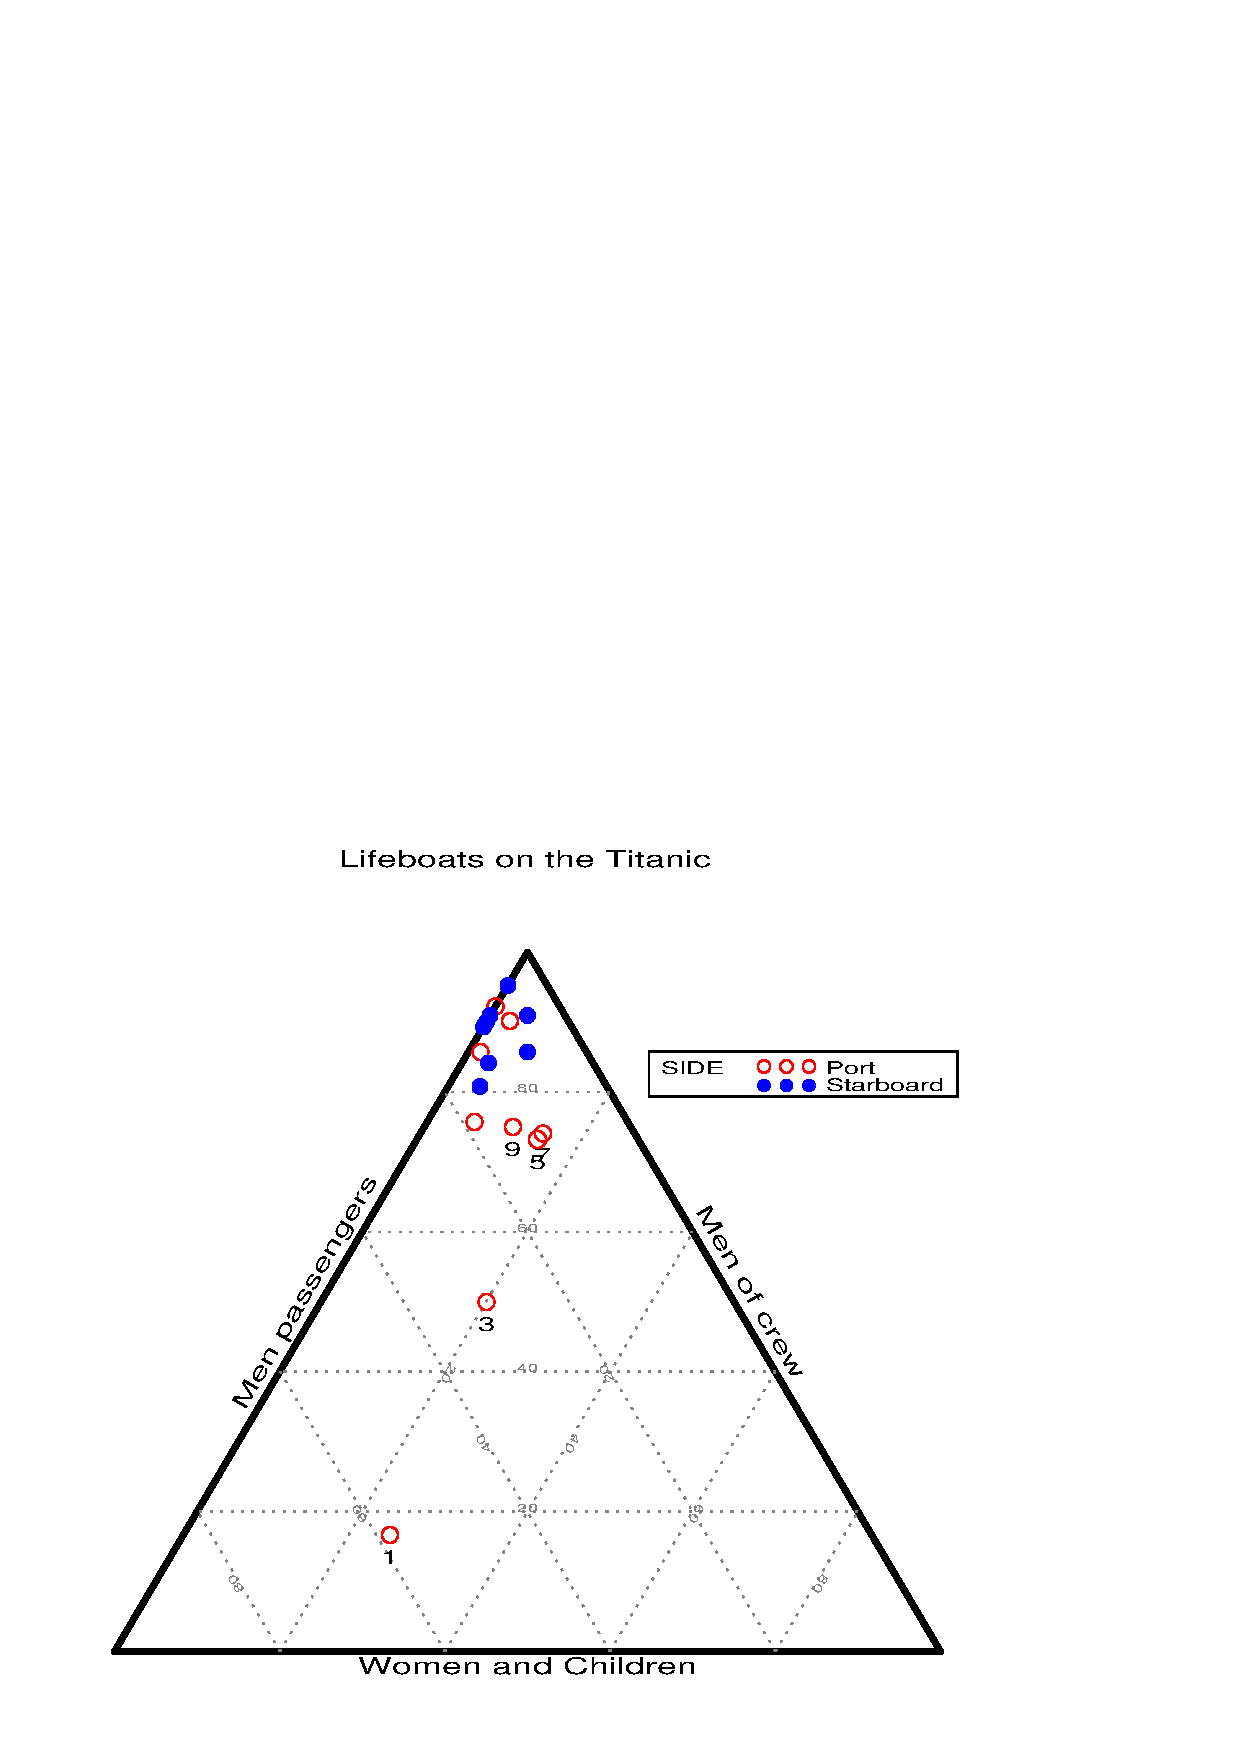
\includegraphics[scale=.6]{ch3/fig/lifeboat1}
  \caption[Lifeboats on the \emph{Titanic}]{Lifeboats on the \emph{Titanic},
  showing the composition of each boat.  Boats with more than 10\% male
  passengers are labeled.}%
  \label{fig:lifeboat1}
\end{figure}

The result, shown in \figref{fig:lifeboat1}, makes it immediately apparent
that many of the boats launched from the port side differ substantially
from the remaining boats, whose passengers were almost entirely women
and children.  Boat 1 had only 20\% (2 out of 10) women and children, while the percentage for boat 3 was only 50\% (25 out of 50).


The triplot scales the numbers for each observation to sum to 1.0,
so differences in the total number of people on each boat
cannot be seen in \figref{fig:lifeboat1}.
The total number reported loaded is plotted against launch time in \figref{fig:lifeboat2},
with a separate regression line fit to the data for the port and starboard
sides.
It seems clear that the rescue effort began in panic on the port side,
with relatively small numbers loaded, and (from \figref{fig:lifeboat1}),
small proportions of women and children.
But the loading regime improved steadily over time.
The procedures began more efficiently on the starboard side
and the numbers loaded increased only slightly, though still
with large variability from boat to boat.
\begin{figure}[htb]
  \centering
  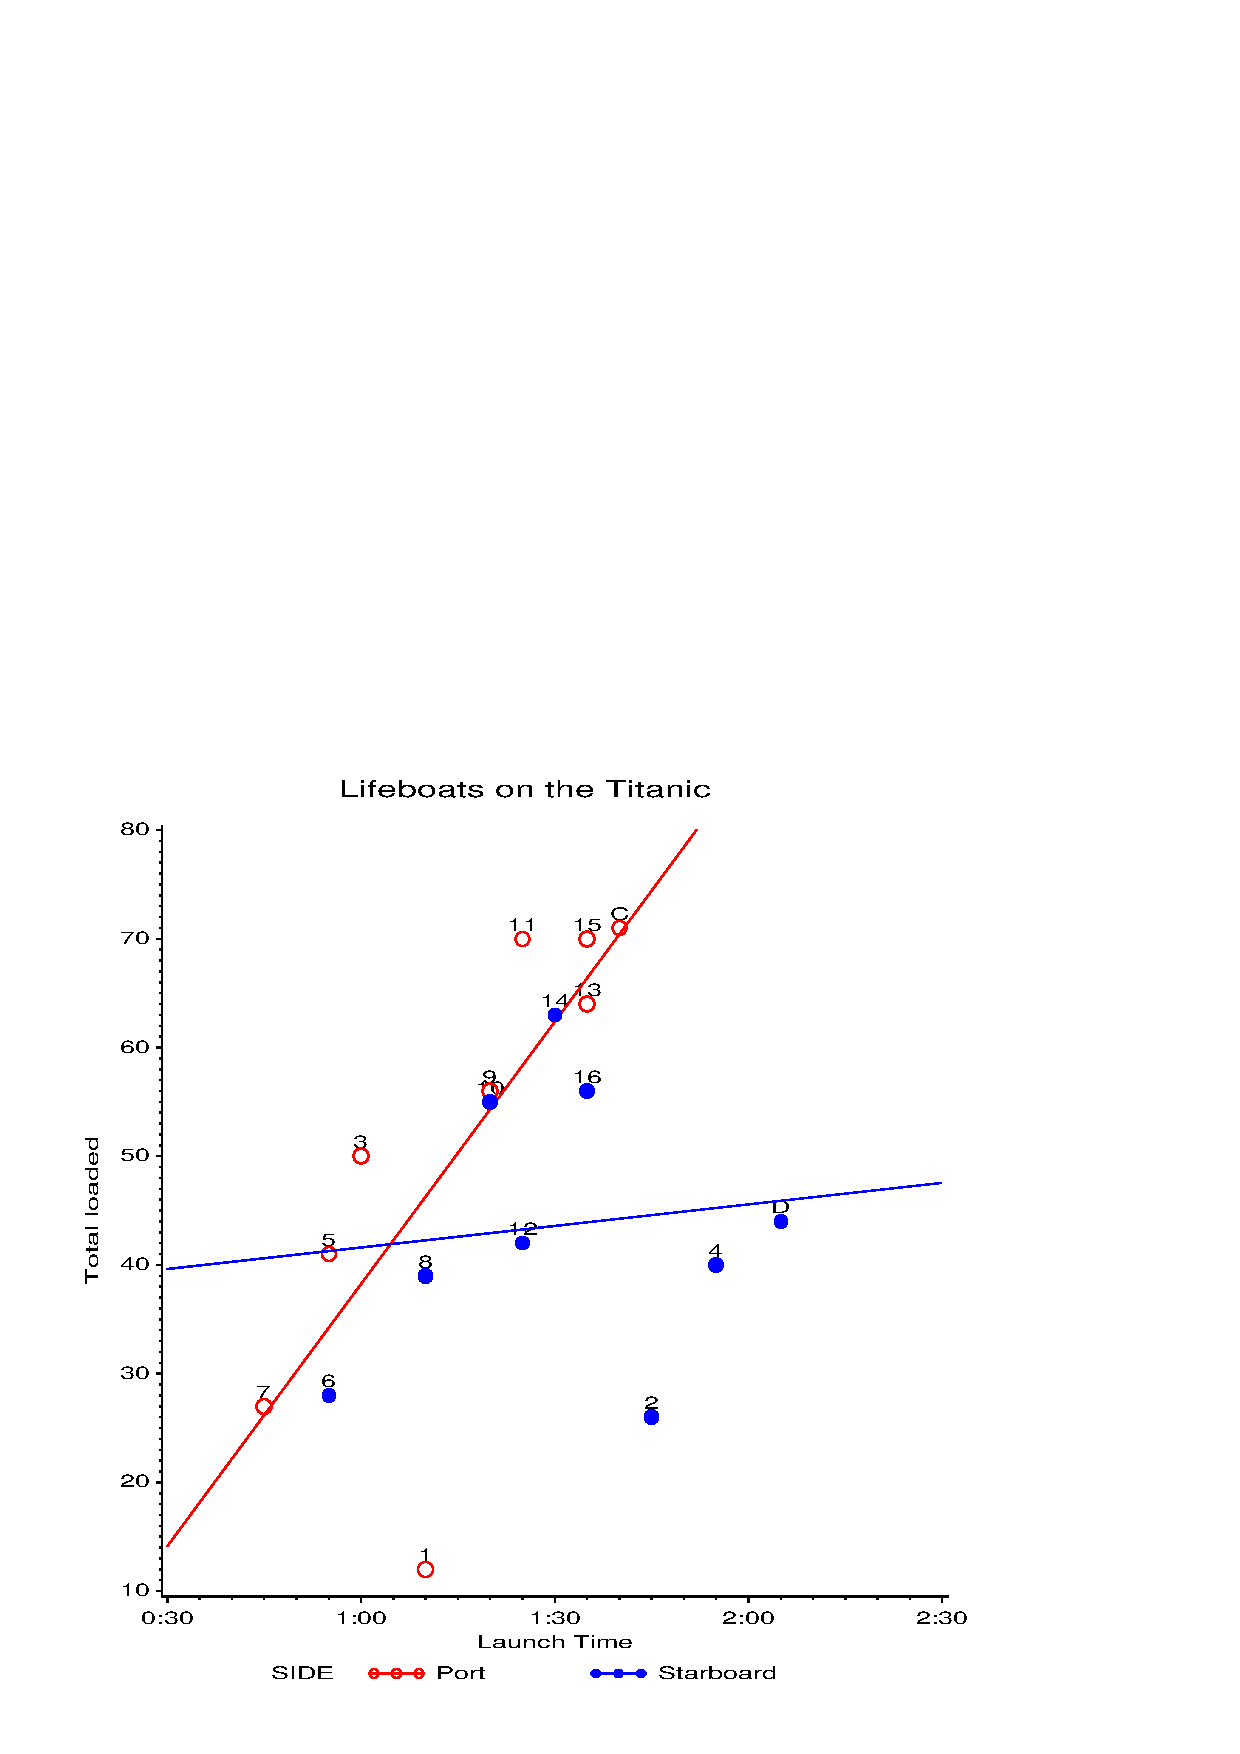
\includegraphics[scale=.6]{ch3/fig/lifeboat2}
  \caption[Lifeboats on the \emph{Titanic}]{Lifeboats on the \emph{Titanic},
  showing the numbers loaded on each boat.
  Regression lines for each side indicate a difference in regimes for
  the port and starboard sides.}%
  \label{fig:lifeboat2}
\end{figure}
\end{Example}
